\chapter{Se rep\'erer dans l'espace}


\section{Le syst\`eme de coordonn\'ees}


\subsection{Le rep\`ere ''main droite''}

Le rep\`ere est orthogonal et orthonorm\'e (les axes/les vecteurs directeurs de ces axes sont perpendiculaires les uns aux autres et de longueur 1)



\subsection{Pourquoi main droite ?}

Regardez votre main droite.
\begin{itemize} 
\item Votre pouce repr\'esente l'axe X, 
\item votre index repr\'esente l'axe Y,
\item votre majeur repr\'esente l'axe Z. 
\end{itemize}

La direction dans laquelle pointe chacun de vos doigts d\'efinit le sens de chaque axe.

Image utilisateur cf(\url{fr.openclassrooms.com/informatique/cours/decouvrez-ogre-3d/le-systeme-de-coordonnees-1})





\subsection{Rep\`ere local, rep\`ere absolu}

Pour l'instant, nous n'avons toujours pas d\'efini comment le rep\`ere \'etait plac\'e dans la sc\`ene. C'est une question de convention adopt\'ee pour les applications 3D	pour le rep\`ere de la sc\`ene:
\begin{itemize}
\item l'axe Y dirig\'e vers le haut 
\item les axes X et Z dans un plan horizontal.
\end{itemize}

Seulement\footnote{comment faire pour sauter une ligne avant le ''Seulement''?}, la sc\`ene n'est pas la seule \`{a} avoir son rep\`ere. En effet, chaque objet poss\`ede son propre rep\`ere appel\'e rep\`ere local. Lorsque l'objet se d\'eplace ou tourne sur lui-m\^eme, le rep\`ere local fait de m\^eme. L'orientation du rep\`ere local est la suivante: 
\begin{itemize}
\item l'axe Y est dirig\'e vers le haut de l'objet, pour la sc\`ene, 
\item l'axe X est dirig\'e vers sa droite
\item l'axe Z vers l'arri\`ere de l'objet.
\end{itemize}
	


Ci-dessous\footnote{comment faire pour sauter une ligne avant le ''Ci-dessous''?}, j'ai repr\'esent\'e en noir le rep\`ere de la sc\`ene, et en bleu le rep\`ere local de la voiture, en respectant la convention que j'ai donn\'ee.
Image utilisateur cf(\url{fr.openclassrooms.com/informatique/cours/decouvrez-ogre-3d/le-systeme-de-coordonnees-1})

Nous verrons \`{a} quoi servent ces diff\'erents rep\`eres lorsque l'on commencera \`{a} d\'eplacer nos objets.








\subsection{Yaw, pitch, roll}

yaw pitch roll sont les d\'esignations anglaises pour les rotations autour des axes Y, X et Z respectivement. On peut traduire ces termes par lacet (yaw), tangage (pitch) et roulis (roll), qui sont utilis\'es par exemple en a\'eronautique ou en navigation.

Ces trois termes se retrouveront dans les noms qu'Ogre donne aux m\'ethodes permettant d'effectuer des rotations. 

Voici tout de suite un sch\'ema illustrant les rotations qui s'appliquent \`{a} chaque axe:

Image utilisateur cf(\url{fr.openclassrooms.com/informatique/cours/decouvrez-ogre-3d/le-systeme-de-coordonnees-1})


Tout comme l'orientation des axes de notre rep\`ere, il y a un sens direct et un sens indirect pour les rotations! Vous tournerez dans le sens direct lors  d'une rotation contraire\footnote{''rotation contraire'' <-> ''sens direct'', est ce correct?} au sens des aiguilles d'une montre.

Pour effectuer une rotation, on appelle la m\'ethode correspondante pour le noeud:
\begin{lstlisting}
	node->yaw(Radian(Math::PI));
\end{lstlisting}

Ceci fera faire un demi-tour au noeud par rapport \`{a} son axe vertical tandis que les m\'ethodes pitch() et roll() s'utilisent de fa\c{c}on analogue pour les autres axes.

La rotation se fait par d\'efaut par rapport au rep\`ere local. Il faut renseigner le second param\`etre si vous voulez qu'il en soit autrement (voir la section suivante).

Les angles doivent \^etre entr\'es en radians. Pour utiliser tout de m\^eme des degr\'es dans Ogre, vous devrez utiliser la classe Degree. La ligne de code pr\'ec\'edente est \'equivalente \`{a} ceci:
\begin{lstlisting}
	node->yaw(Degree(180));
\end{lstlisting}









\section{D\'eplacer des objets}




\subsection{Bouger un noeud de sc\`ene}

Nous allons maintenant d\'eplacer notre t\^ete d'ogre pour v\'erifier la th\'eorie et enfin sortir notre t\^ete de terre!

Pour cela, nous allons donc passer par le noeud auquel est rattach\'e notre mesh. Celui-ci poss\`ede deux m\'ethodes qui peuvent nous servir.




\subsection{setPosition()}

La m\'ethode setPosition() prend en param\`etres les trois coordonn\'ees X, Y et Z du point auquel on d\'esire placer le noeud. On peut aussi lui passer un Vector3, qui contiendra lui-m\^eme ces coordonn\'ees.

Les deux codes suivants sont donc \'equivalents.
\begin{lstlisting}
	Vector3 position = Vector3(30.0, 50.0, 0.0);
	node->setPosition(position);
\end{lstlisting}

ou
\begin{lstlisting}
	node->setPosition(30.0, 50.0, 0.0);
\end{lstlisting}

La t\^ete s'est maintenant d\'eplac\'ee vers la droite de 30 unit\'es et de 50 unit\'es vers le haut.




\subsection{translate()}

La m\'ethode translate() d\'eplace le noeud par rapport \`{a} sa position actuelle plut\^ot que par rapport \`{a} l'origine de la sc\`ene.

Elle prend les m\^emes param\`etres que la m\'ethode setPosition(), mais avec un param\`etre suppl\'ementaire, d\'efini par d\'efaut, indiquant le noeud par rapport auquel on va se d\'eplacer.
\begin{lstlisting}
	node->translate(-30.0, 50.0, 0.0);
\end{lstlisting}

En ajoutant cette ligne apr\`es la pr\'ec\'edente, notre objet se retrouve donc maintenant \`{a} la position (0, 100, 0) dans la sc\`ene, ce qui est suffisant pour qu'il surplombe son petit jardin.

Image utilisateur

Le param\`etre suppl\'ementaire (par rapport \`{a} setPosition) permet de d\'efinir par rapport \`{a} quel rep\`ere on va d\'eplacer le noeud.

Les trois valeurs possibles sont:
\begin{lstlisting}
    Node::TS_LOCAL //va deplacer le noeud par rapport au repere local
    Node::TS_PARENT //va deplacer le noeud au repere du noeud parent
    Node::TS_WORLD //va deplacer le noeud au repere de la scene, qui est le repere absolu.
\end{lstlisting}\footnote{Pour présenter les 3 valeurs possibles ne devrais je pas faire une liste itemize plutot que d'utiliser un bloc de code?}



\subsection{Concr\`etement, \c{c}a veut dire quoi ?}

Tout \`{a} l'heure, lorsque l'on a effectu\'e une translation, on l'a fait par d\'efaut par rapport au rep\`ere TS\_WORLD, c'est-\`{a}-dire avec les axes tels que je vous les ai pr\'esent\'es pr\'ec\'edemment. Maintenant, nous pouvons d\'eplacer notre noeud par rapport au rep\`ere local de son noeud p\`ere par exemple, ou bien m\^eme par rapport \`{a} son propre rep\`ere local.

Mais \`{a} quoi \c{c}a sert de s'emb\^eter avec ces param\`etres ? On risque de faire des erreurs si l'on se place par rapport \`{a} un rep\`ere diff\'erent de la sc\`ene!

Prenons un exemple. Vous avez un vaisseau spatial qui peut se trouver dans n'importe quelles position et orientation de l'espace. Comment savoir facilement dans quelle direction je dois faire ma translation pour qu'on le voit aller en avant ?

R\'eponse: je n'ai pas \`{a} m'en occuper! En effet, l'axe qui va de l'avant vers l'arri\`ere du vaisseau est l'axe Z, dans son rep\`ere local. Par cons\'equent, je n'ai qu'\`{a} dire \`{a} mon vaisseau d'avancer le long de l'axe Z (dans le sens n\'egatif pour aller \`{a} l'avant) par rapport \`{a} son rep\`ere local. Et Ogre s'occupera gentiment de faire les calculs pour placer mon vaisseau correctement dans la sc\`ene.

Image utilisateur \url{http://fr.openclassrooms.com/informatique/cours/decouvrez-ogre-3d/deplacer-des-objets}

Si vous avez compris cela, le param\`etre TS\_PARENT devrait suivre tout seul. Reprenons notre engin spatial.
Sur ce vaisseau, on trouve R2D2 en train de se d\'eplacer vers la droite, correspondant donc \`{a} l'axe X local du noeud du vaisseau. Pour effectuer cette translation, je n'ai qu'\`{a} demander \`{a} Ogre de d\'eplacer mon robot le long de l'axe des abscisses par rapport au noeud du vaisseau (qui serait logiquement le noeud parent).

Vous commencez \`{a} comprendre l'int\'er\^et des relations de parent\'e entre les noeuds ?









\section{La cam\'era}


La cam\'era, c'est l'\'el\'ement qui d\'efinit la position de notre point de vue dans la sc\`ene, dans quelle direction on regarde, mais aussi jusqu'\`{a} quelle distance il est possible de voir s'afficher les objets \'eloign\'es.

Comme tous les \'el\'ements de base, un attribut cam\'era est pr\'esent dans la classe ExampleApplication. Sans elle nous n'aurions pas encore pu voir notre sc\`ene, vu que nous n'avons rien fait pour la cr\'eer!



\subsection{Cr\'eation}

La cam\'era est cr\'e\'ee par la m\'ethode  createCamera() de la classe ExampleApplication, nous allons tout de suite red\'efinir cette m\'ethode pour partir sur des bases connues. L'attribut correspondant \`{a} la cam\'era est appel\'e mCamera, nous pouvons donc l'utiliser pour cr\'eer notre cam\'era.

Comme c'est un objet qui se trouve dans la sc\`ene, nous allons passer par le sceneManager. Comme pour les noeuds ou les entit\'es, vous pourrez donner un nom \`{a} votre cam\'era sous forme d'une cha\^ine de caract\`eres.

Ajoutez la m\'ethode createCamera() \`{a} votre classe PremiereApplication et ajoutez-y la ligne suivante.

\begin{lstlisting}
	mCamera = msceneMgr->createCamera(''Ma Camera'');
\end{lstlisting}





\subsection{Placement}

Maintenant, il va nous falloir placer la cam\'era et l'orienter. Le placement se fait avec la m\'ethode setPosition(). 

La seconde m\'ethode utilis\'ee s'appelle lookAt() et, comme son nom l'indique, elle permet de d\'eterminer le point de la sc\`ene que regarde notre cam\'era. On lui fournit un Vector3 ou bien trois r\'eels correspondant aux coordonn\'ees d\'esir\'ees.

\begin{lstlisting}
	//placement de la camera
	mCamera->setPosition(Vector3(-100.0, 150.0, 200.0));
	//point de la scene que regarde notre camera
	mCamera->lookAt(Vector3(0.0, 100.0, 0.0));
\end{lstlisting}


Enfin, on peut aussi indiquer les distances near clip et far clip, qui sont les distances minimale et maximale\footnote{''les distances minimale et maximale'' il faut pas de ''s'' \`{a} ''max/minimale""} auxquelles doit se trouver un objet pour \^etre affich\'e \`{a} l'\'ecran.
\begin{lstlisting}
	mCamera->setNearClipDistance(1);
	mCamera->setFarClipDistance(1000);
\end{lstlisting}




\subsection{Code}

\subsubsection{PremiereApplication.cpp}
\begin{lstlisting}[caption={PremiereApplication.cpp: Cr\'eation de la cam\'era}]

#include "PremiereApplication.h"

void PremiereApplication::createScene()
{
    //creation d une entite
    Entity *head= mSceneMgr->createEntity("Tete", "ogrehead.mesh" );
    
    //creation d un noeud
    SceneNode *node= mSceneMgr->getRootSceneNode( )->createChildSceneNode( "nodeTete " , Vector3::ZERO, Quaternion::IDENTITY);
    
    node->yaw(Radian(Math::PI));
    node->yaw(Radian(Math::PI));

    //setPosition place le noeud aux coord passees en parametres
    Vector3 position = Vector3(30.0, 50.0, 0.0);
    node->setPosition(position);

    node->setPosition(30.0, 50.0, 0.0); 
    /*equivalent a
    Vector3 position = Vector3(30.0, 50.0, 0.0);
    node->setPosition(position);
    */

    //deplace le noeud par rapport a sa position actuelle
    node->translate(-30.0, 50.0, 0.0); //par defaut la trnslt se fait par rap a TS_WORLD
   
    //attachement de l entite au noeud
    node->attachObject ( head );

    //creation d un plan
    Plane plan(Vector3::UNIT_Y, 0);

    //creation d un mesh cad l objet 3d visible ds la scene
    MeshManager::getSingleton().createPlane("sol",
                ResourceGroupManager::DEFAULT_RESOURCE_GROUP_NAME,
                plan, 500, 500, 1, 1, true, 1, 1, 1, Vector3::UNIT_Z); 

    //entite qui representera le plan
    Entity *ent= mSceneMgr->createEntity("EntiteSol", "sol");

    //ajout du materiau a l entite
    ent->setMaterialName("Examples/GrassFloor");//texture de pelouse
    /*les differents materiaux sont sous /media/materials/scritps, par ex:
    ent->setMaterialName("Examples/WaterStream");//texture d eau animee*/

    //creation d un noeud
    node = mSceneMgr->getRootSceneNode()->createChildSceneNode();
    node->attachObject(ent);
}

/*definit la position de notre point de vue*/
void PremiereApplication::createCamera()
{
    //creation de la camera
    mCamera = mSceneMgr->createCamera("Ma Camera");

    //position de la camera
    mCamera->setPosition(Vector3(-100.0, 150.0, 200.0));

    //permet de determiner le point de la scene que regarde notre camera
    mCamera->lookAt(Vector3(0.0, 100.0, 0.0));

    //definition des distances de near clip et de far clip, qui
    //sont les distances minimale et maximale auxquelles doit se
    //trouver un objet pour être affichr à l'écran.
    mCamera->setNearClipDistance(1);
    mCamera->setFarClipDistance(1000);
}

\end{lstlisting}



\subsubsection{PremiereApplication.h}
\begin{lstlisting}[caption={PremiereApplication.h: Cr\'eation de la cam\'era}]
using namespace std;

#include <ExampleApplication.h>

class PremiereApplication : public ExampleApplication
{
public:
    void createScene();
    void createCamera();
};

\end{lstlisting}


\subsubsection{main.cpp}
\begin{lstlisting}[caption={main.cpp: Cr\'eation de la cam\'era}]
#include <Ogre.h>

#include "PremiereApplication.h"

#if OGRE_PLATFORM == PLATFORM_WIN32 || OGRE_PLATFORM == OGRE_PLATFORM_WIN32
#define WIN32_LEAN_AND_MEAN
#include "windows.h"

INT WINAPI WinMain(HINSTANCE hInst, HINSTANCE, LPSTR strCmdLine, INT)
#else
int main(int argc, char **argv)
#endif
{

    PremiereApplication app;
    
    try {
      app.go();
    } catch(Ogre::Exception& e) {
#if OGRE_PLATFORM == OGRE_PLATFORM_WIN32
        MessageBoxA(NULL, e.getFullDescription().c_str(), "An exception has occurred!", MB_OK | MB_ICONERROR | MB_TASKMODAL);
#else
        fprintf(stderr, "An exception has occurred: %s\n",
            e.getFullDescription().c_str());
#endif
    }

    return 0;
}
\end{lstlisting}




































\section{Le viewport}

Une zone de rendu est une portion de l'\'ecran sur laquelle est affich\'ee ce que voit la cam\'era. La gestion de l'affichage dans une zone de rendu est \`{a} la charge de la classe Viewport.

Cette gestion de la zone de rendu a cel\`{a} d'important que:
\begin{itemize}
\item la fa\c{c}on dont la cam\'era rend \`{a} l'\'ecran ce qu'elle voit ne d\'epend pas que d'elle. En effet, la taille de votre zone de rendu et son format seront r\'epercut\'es sur la portion de sc\`ene qu'il vous sera donn\'e de voir. Si l'on ne tenait pas compte de ces param\`etres, on pourrait obtenir une image aplatie si l'on \'elargissait la zone de rendu, ou bien au contraire compress\'ee si l'on diminuait la largeur en laissant la hauteur constante.
\item sur une m\^eme \'ecran, vous pouvez afficher le rendu de plusieurs cam\'eras dans la sc\`ene, voire des cam\'eras de diff\'erents sceneManager.
\end{itemize}


Nous allons red\'efinir la m\'ethode createViewports() qui s'occupait jusqu'alors de ce travail pour nous. On commence par ajouter une vue:

\begin{lstlisting}
	Viewport *vue = mWindow->addViewport(mCamera);
\end{lstlisting}

Ici, mWindow est la fen\^etre de notre application Ogre, c'est une instance de la classe RenderWindow dont nous verrons les d\'etails dans un prochain chapitre. La m\'ethode addViewport permet donc d'ajouter une vue, seul son premier argument est obligatoire. Ce premier argument est la cam\'era \`a partir de laquelle est rendu la sc\`ene affich\'ee dans la vue.

Nous allons faire co\"incider le rapport largeur/hauteur de notre cam\'era avec celui du Viewport, pour avoir une image non d\'eform\'ee:
\begin{lstlisting}
mCamera->setAspectRatio(Real(vue->getActualWidth()) / Real(vue->getActualHeight()));
\end{lstlisting}

On applique un cast vers le format Ogre::Real pour obtenir un ratio d\'ecimal. Dans le cas contraire, le ratio serait tronqu\'e pour \^etre entier et la t\^ete de notre ogre favori serait d\'eform\'ee.

Sachez aussi que c'est le Viewport qui d\'efinit la couleur de fond de la sc\`ene que vous voyez. 
\begin{lstlisting}
vue->setBackgroundColour(ColourValue(0.0, 0.0, 1.0));
\end{lstlisting}

Voici donc ma m\'ethode createViewports() au complet:
\begin{lstlisting}[caption={Cr\'eation d'un viewport}]
void PremiereApplication::createViewports()
{
    Viewport *vue = mWindow->addViewport(mCamera);
    
    
    //nous faisons coincider le rapport largeur / hauteur de 
    //notre camera avec celui du Viewport, pour avoir 
    //une image non deformee
    mCamera->setAspectRatio(Real(vue->getActualWidth()) / Real(vue->getActualHeight()));
    
    //couleur de fond de la vue
    vue->setBackgroundColour(ColourValue(0.0, 0.0, 1.0));
}
\end{lstlisting}


Maintenant, notre sc\`ene poss\`ede un magnifique ciel fond bleu.









\subsection{Plusieurs viewports}
La m\'ethode addViewport permet d'ajouter des vues \`a notre sc\`ene, on peut donc avoir plusieurs vues \`a l'\'ecran. Pour cel\`a il faut renseigner les autres param\`etres de la m\'ethode addViewport.\newline
Voici le \href{http://www.ogre3d.org/docs/api/1.9/classOgre_1_1RenderTarget.html#a1a558e64db9dfd7cc4cec4547fca0e39}{prototype} de la m\'ethode addViewport.


\begin{lstlisting}[caption={Prototype de addViewport}]
virtual Viewport* Ogre::RenderTarget::addViewport(
	 	Camera *  	cam,
		int  	ZOrder = 0,
		float  	left = 0.0f,
		float  	top = 0.0f,
		float  	width = 1.0f,
		float  	height = 1.0f 
		) 
\end{lstlisting}

Les param\`etres sont les suivants\footnote{d'autres essais et recherches seraient n\'ecessaires pour la pleine compr\'ehension de ces param\`etres}:
\begin{itemize}
\item ZOrder: ordre relatif des vues les unes par rapport aux autres, les Z-orders les plus \'elev\'es sont au-dessus des autres. Le nombre donn\'ee est pas important en lui-m\^eme car il s'agit d'une relation avec les autres Z-order, ainsi peut-on utiliser des nombres qui ne suivent pas.
\item left: la position relative de la gauche du viewport sur la cible\footnote{''cible'' est visiblement le viewport principal} (entre 0 et 1).
\item top: la position relative du haut du viewport sur la cible (entre 0 et 1).
\item width: la largeur relative du viewport sur la cible (entre 0 et 1).
\item height: la hauteur relative du viewport sur la cible (entre 0 et 1).
\end{itemize}


	
\subsubsection{Code: 2 vues}
Le code suivant permet la cr\'eation de deux viewports:


\begin{lstlisting}[caption={createViewports: cr\'eation de plusieurs vues}]
void PremiereApplication::createViewports()
{
    //la creation du Viewport "principal"
    Viewport *vue = mWindow->addViewport(mCamera, 0, 0, 0, 0.8, 0.8);
    mCamera->setAspectRatio(Real(vue->getActualWidth()) /  Real(vue->getActualHeight()));
    vue->setBackgroundColour(ColourValue(0.980, 0.502, 0.447)); //saumon

   // creation d'un second viewport
   Viewport* vue2 = mWindow->addViewport(mCamera, 1, 0.5, 0, 0.2, 0.2);
   vue2->setBackgroundColour(ColourValue(0.561, 0.737, 0.561 ));  //darkseagreen
}
\end{lstlisting}

Et j'obtiens:
	\begin{center}
	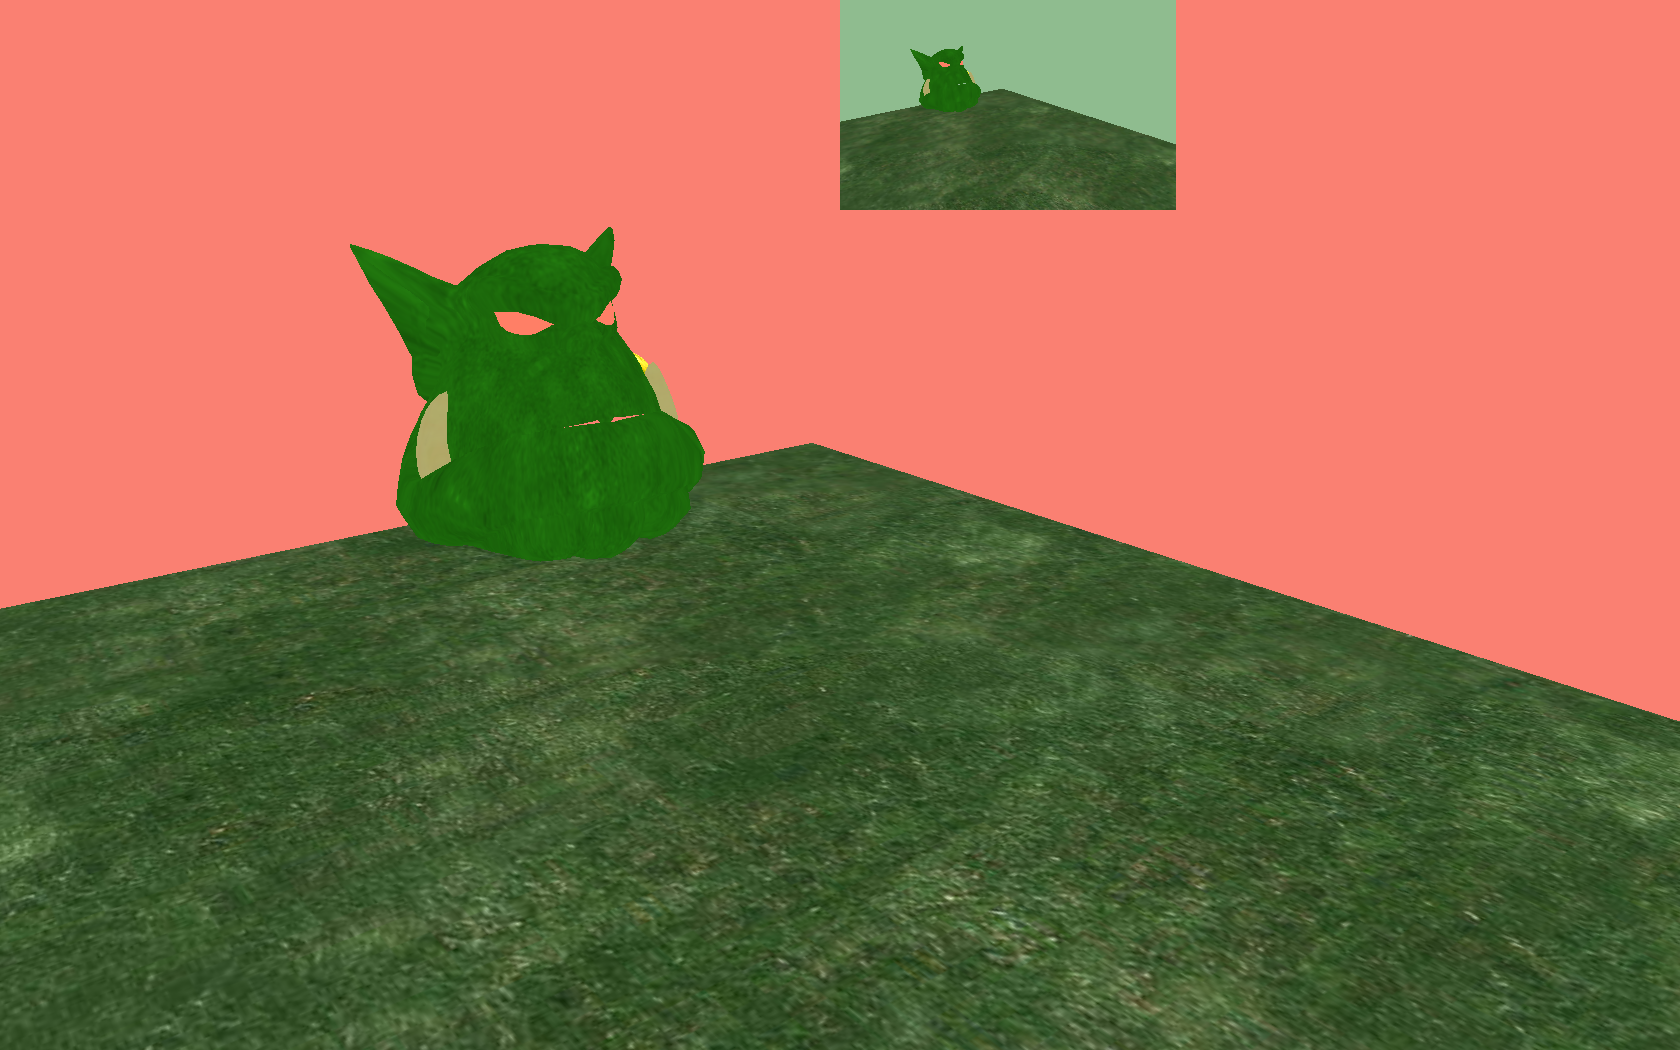
\includegraphics[scale=0.25]{Base_de_Ogre/Se_reperer_ds_l_espace/Images/plusieursViewport.png} 
	\end{center}






\subsubsection{Code: 3 vues}
Le code suivant permet la cr\'eation de deux viewports:


\begin{lstlisting}[caption={createViewports: cr\'eation de plusieurs vues}]



void PremiereApplication::createViewports()
{
    //Viewport "principal"
    Viewport *vue = mWindow->addViewport(mCamera);
    mCamera->setAspectRatio(Real(vue->getActualWidth()) /  Real(vue->getActualHeight()));
    vue->setBackgroundColour(ColourValue(0.980, 0.502, 0.447)); //saumon

	//seconde vue
    Viewport* vue2 = mWindow->addViewport(mCamera, 1, 0.5, 0, 0.8, 0.8);
    vue2->setBackgroundColour(ColourValue(0.561, 0.737, 0.561 ));  //darkseagreen

	//troisieme vue
	Viewport* vue3 = mWindow->addViewport(mCamera, 4, 0, 0.4, 0.2, 0.2);
    vue3->setBackgroundColour(ColourValue(0.878, 1.000, 1.000));  //
}
\end{lstlisting}

Et j'obtiens:
	\begin{center}
	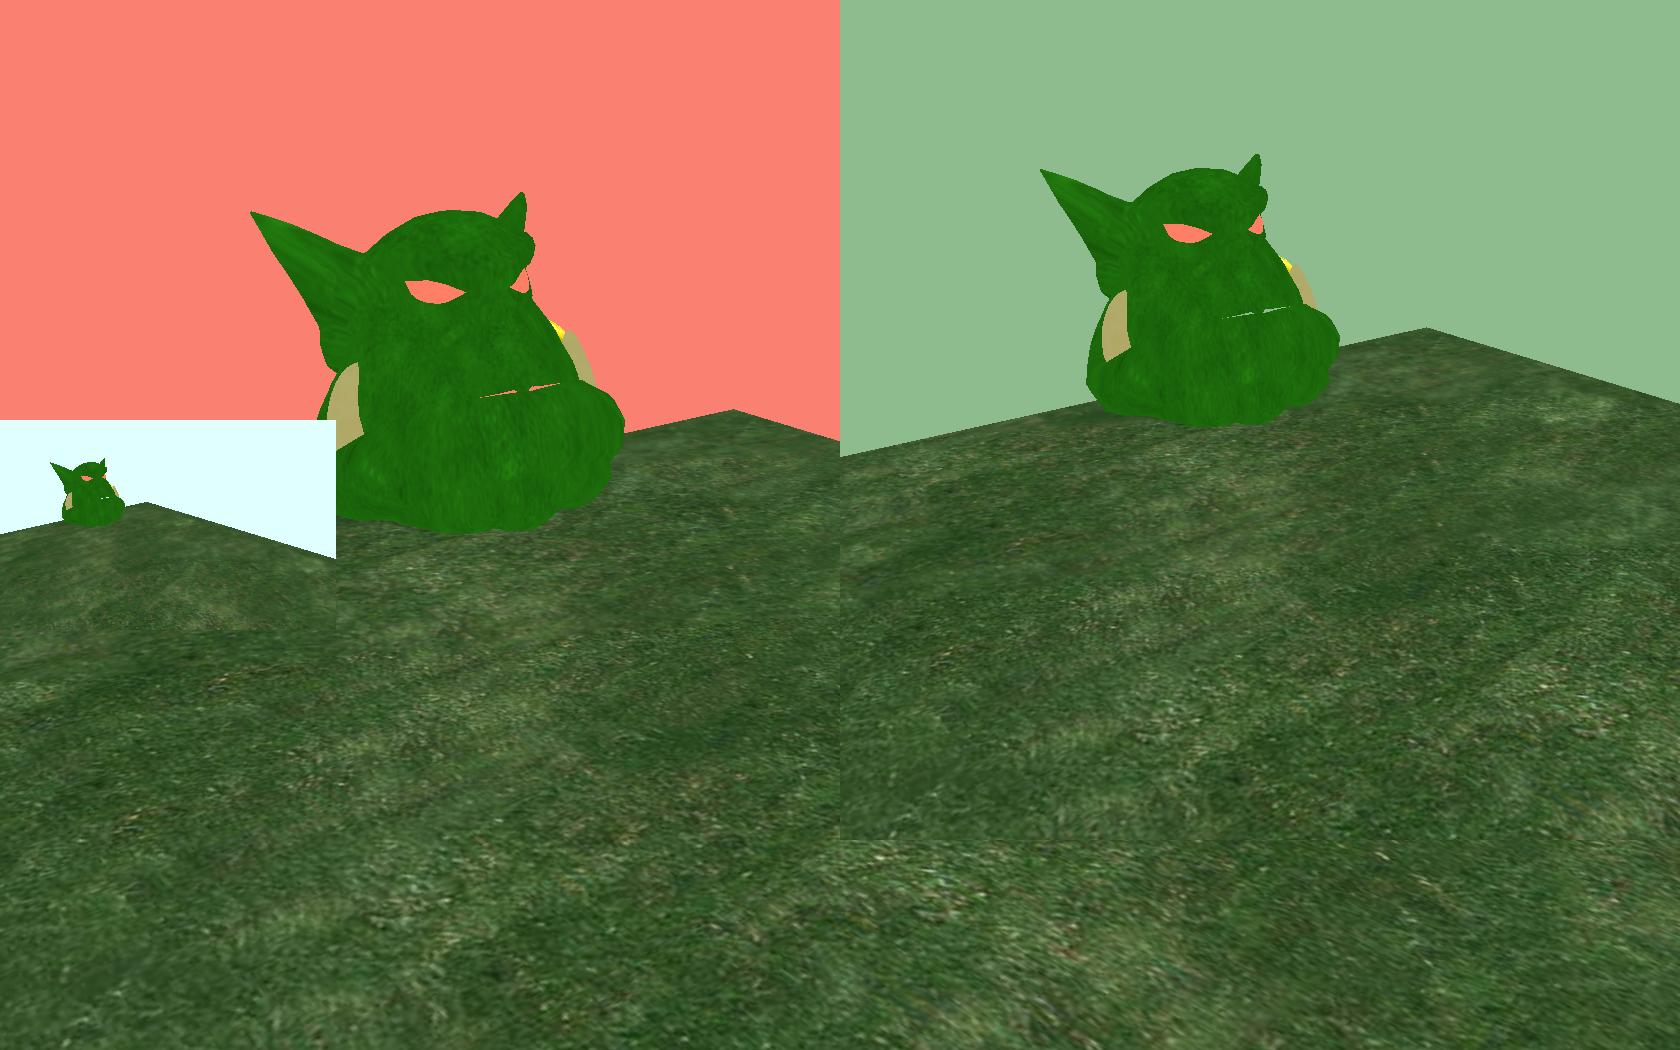
\includegraphics[scale=0.25]{Base_de_Ogre/Se_reperer_ds_l_espace/Images/plusieursViewport2.png} 
	\end{center}























